\section{Algoritmos}
\label{sec:algoritmos}
\subsection{Introducción}
En esta sección vamos a explicar que algoritmos se han usado después del pre-procesamiento inicial.\\
Existe un teorema llamado\textbf{ \textit{No-Free-Lunch}} que afirma no existe un algoritmo que resuelva los problemas de machine learning mejor que otro.\\
Partiendo de esta idea, el objetivo principal de esta sección es el de comprobar el comportamiento de una serie de modelos elegidos. \\
De estos modelos, algunos se adaptaran mejor que otros para los datos con los que se trabajan. Una vez analizado el comportamiento, podremos decidir que algoritmos vamos a usar y que algoritmos van a ser descartados. \\
\linebreak
Para el caso especifico con el que se está trabajando, vemos que es un problema bastante peculiar, ya que esta formado por varias variables objetivo de tipo ordinal, añadiendo una nueva característica siendo esta la\textbf{media} de estas variables.\\
Para esta sección, se ha usado la media y se ha planteado un problema de \textbf{regresión}, en el que algoritmo, dada una entrada predecirá que valor medio de emprendimiento tiene esa persona.

\subsection{Métricas}
Para comprobar el comportamiento de nuestro modelo se usan \textbf{métricas}.  Las métricas que se han usado son \textit{\textbf{Coeficiente de determinación}} (se denota como $R^2$), \textit{\textbf{Desviación de Poisson}} y \textit{\textbf{Error cuadrático medio}}
\subsubsection{Coeficiente de determinación}
Se define como \textbf{coeficiente de determinación} como la proporción de la varianza total explicada por la variables independientes del modelo. Proporciona una indicación de como de bueno es un ajuste y por tanto, una medida de como de bueno es el modelo cuando predice nuevas muestras.\\
\linebreak
Matemáticamente, se define el coeficiente de determinación como:
\[
	R^2 (y, \hat{y}) = 1 - \frac{\sum_{i=1}^{n}(y_i - \hat{y}_i)^2}    {\sum_{i=1}^{n} (y_i - \overline{y})^2}
\]

Donde:
\begin{itemize}
	\item $y$ es el conjunto de valores reales para las variables objetivo.
	\item $\hat{y}$ es el valor predicho para los valores objetivo.
	\item $\hat{y}_i$ es la predicción de la  i-ésima muestra.
	\item $y_i$ es el valor real de la i-ésima muestra.
	\item $\overline{y} = \frac{1}{n} \sum_{i=1}^{n} y_i$.
	\item $n$ es el numero de muestras del conjunto.
\end{itemize}
insertar graficos explicando varianza,  etc
\subsubsection{Desviación de Poisson}
\subsubsection{Error cuadrático medio}
El error cuadrático medio de un estimador mide el promedio de los errores al cuadrado.  \\
Matemáticamente, se define el error cuadrático medio como:
\[
	MSE(y,\hat{y}) = \frac{1}{n} \sum_{i=1}^{n} (y_i - \hat{y}_i) ^2
\]
Donde:
\begin{itemize}
	\item $y$ es el conjunto de valores reales para las variables objetivo.
	\item $\hat{y}$ es el valor predicho para los valores objetivo.
	\item $\hat{y}_i$ es la predicción de la  i-ésima muestra.
	\item $y_i$ es el valor real de la i-ésima muestra.
	\item $n$ es el numero de muestras del conjunto.
\end{itemize}
\subsubsection{Conjuntos de validación}
Para ver el comportamiento de un modelo, se puede definir un conjunto de entrenamiento para entrenar el modelo que se ha seleccionado y un conjunto de test para comprobar el comportamiento con datos que el algoritmo no conoce.  Aunque a primera vista esta parece una técnica correcta, tiene varios inconvenientes:
\begin{itemize}
	\item Cuando se ajustan los hiper-parámetros de los modelos,  se podría llegar a ajustar el modelo al conjunto de test, produciendo un sobre-ajuste.
	\item Solo se esta usando una parte de los datos para validar el modelo, nada asegura que el conjunto de test sea representativo del conjunto de datos con el que se está trabajando.
\end{itemize}
Para solventar estas y algunos otros problemas que que tiene esta metodología, se usa la \textbf{validación cruzada}.\\
\linebreak
En vez de usar el conjunto de entrenamiento para entrenar un único modelo, se divide el conjunto de entrenamiento en $k$ partes, entrenando $k$ modelos usando $k-1$ subconjunto y usando el restante como de test. \\
 \begin{figure}[!htbp]
	\centering
	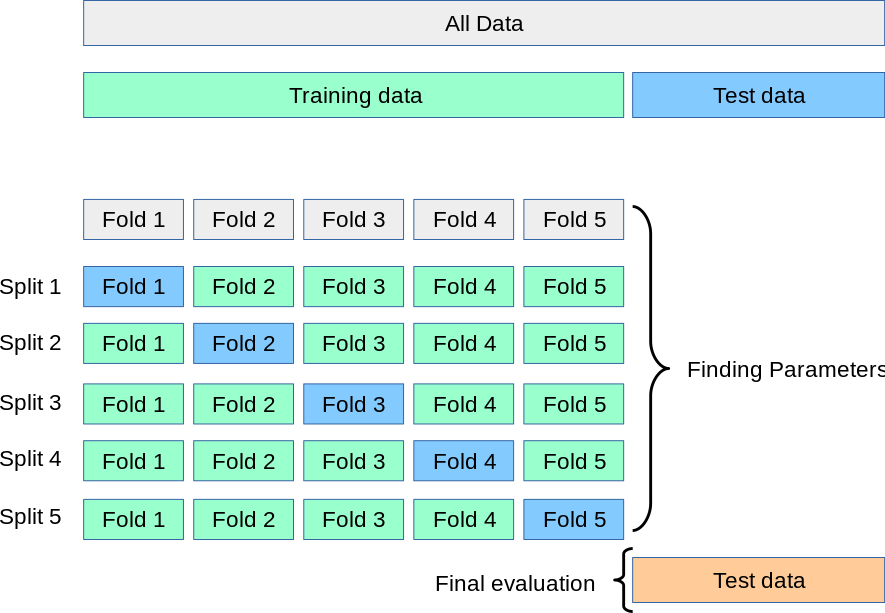
\includegraphics[scale=0.4]{grid_search_cross_validation.png}
	\caption{Ejemplo de validación cruzada con $k=5$}
	\label{fig:cross-validation}
\end{figure}
\linebreak
Como se aprecia en la figura \ref{fig:cross-validation},  se ha dividido el conjunto de datos en 5 conjuntos (folds), usando en cada iteración 4 para entrenar el modelo y uno para verificar con datos que el modelo no ha visto. Finalmente, se usa el conjunto de test (habiendo entrenado previamente el modelo con todo el conjunto de entrenamiento).
\subsubsection{Gráficos}
Además del uso de las métricas mencionadas previamente, se han creado las siguientes gráficas para visualizar los errores que esta haciendo un modelo en concreto. Esto ayuda a la toma de decisiones en fases siguientes.\\
Las gráficas que se han desarrollado son las siguientes:
\begin{itemize}
	\item Gráfico de dispersión de errores.
	\item Cantidad de errores por rango. (probablemente sea mejor cambiar este nombre, pero es el nombre que se me ocurrió)
\end{itemize}
El gráfico de dispersión de errores consiste en mostrar en la misma gráfica el valor real de las variables objetivo y el valor predicho por nuestro modelo. Esto nos permite ver como de juntos están las predicciones, identificando así en que zonas el algoritmo se está equivocando más frecuentemente.\\
 \begin{figure}[!htbp]
	\centering
	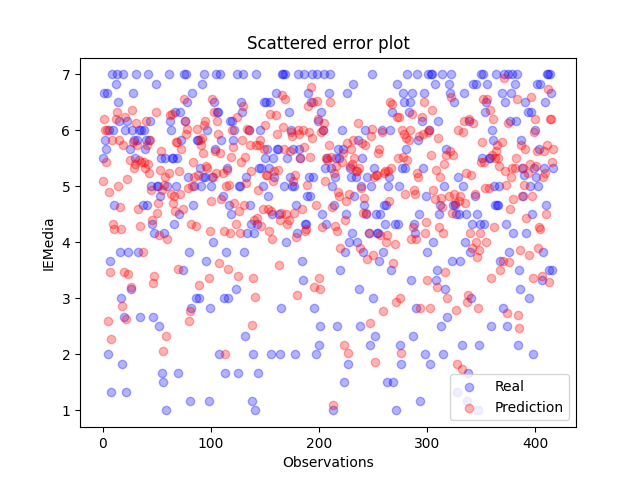
\includegraphics[scale=0.6]{scattered.png}
	\caption{Ejemplo de gráfico de dispersión de errores}
	\label{fig:scattered_example}
\end{figure}
\linebreak
El segundo gráfico consiste en lo siguiente:
Los modelos que han sido entrenados están prediciendo valores medios. El proceso seguido para realizar estos gráficos ha sido el de obtener la diferencia entre los valores reales y los valores predichos. Si esa diferencia es mayor que un umbral (generalmente se ha usado 0.5), esa predicción se ha considerado como error. En ese caso, se ha considerado el valor real redondeado y se han contado el número de errores para cada valor redondeado.\\
Usando esta gráfica, se puede identificar fácilmente en que rangos los modelos están fallando.\\
\linebreak
 \begin{figure}[!htbp]
	\centering
	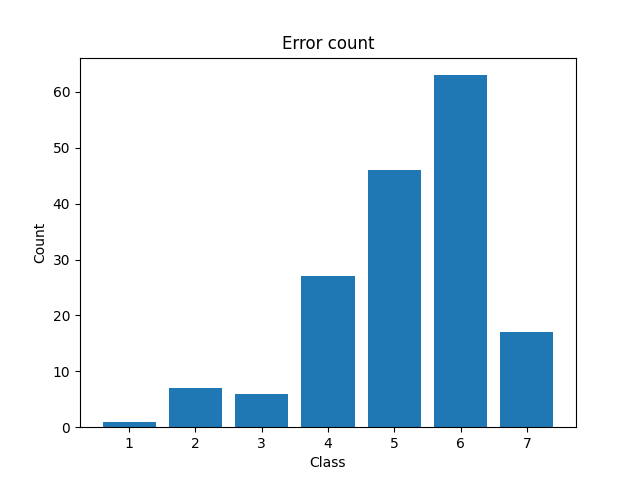
\includegraphics[scale=0.6]{error_hist.png}
	\caption{Ejemplo de gráfico de errores por rango}
	\label{fig:error_hist_example}
\end{figure}
\\
\pagebreak
\subsection{Árboles de decisión}
\label{alg:dec_tree}
Los árboles de decisión son modelos que predicen la variable objetivo usando reglas del tipo \textit{si variable cumple condición entonces } inferidas a partir de los datos con los que se entrena el algoritmo.\\
Los árboles de decisión ofrecen ciertas ventajas:
\begin{enumerate}
	\item Son modelos fáciles de interpretar y pueden ser visualizados.
	\item Son capaces de trabajar con variables categóricas y numéricas.
	\item introducir alguna ventaja más
\end{enumerate}
Sin embargo, estos modelos también presentan ciertas desventajas:
\begin{enumerate}
	\item Algoritmos que tienden al sobre-aprendizaje.
	\item No soportan valores perdidos.
	\item No trabajan bien con conjuntos de datos des-balanceados.
\end{enumerate}
Se ha seleccionado este algoritmo ya que es un algoritmo que a parte de predecir nuevos valores, puede proporcionar información extra sobre conjunto de datos (importancia de variables, variables que definen cierto grupo, etc).
\subsubsection{Procesado de datos}
Antes de ejecutar la fase de entrenamiento, hay que modificar los datos para adaptarlos a las limitaciones que algoritmo impone. En este caso,  los árboles de decisión no admiten valores perdidos y debido a ciertas limitaciones de la librería que se está usando, los árboles de decisión no son capaces de trabajar con variables categóricas.\\
Las modificaciones que se han hecho previamente son: (por orden)
\begin{enumerate}
	\item \textbf{Imputación de valores perdidos}
	\item \textbf{Transformación de variables categóricas a numéricas}
\end{enumerate}
 Por este motivo, se ha tenido que introducir una fase extra transformando las variables categóricas en numéricas.
\subsubsection{Resultados}
Antes de mostrar los resultados, hay que destacar que cuando se entrena un árbol de decisión sin limitar los parámetros, este va a seguir separando los datos de entrenamiento hasta que no pueda realizar más divisiones. Para encontrar el árbol óptimo, primero se ha entrenado el árbol por defecto y se han obtenido los parámetros. Esos parámetros se han establecido como limite, se han entrenado varios árboles con distintos parámetros (sin superar el límite establecido por el primer modelo) y se ha escogido el que mejores resultados obtenía. Los parámetros que mejor resultados dieron son: \\
\begin{itemize}
	\item \textbf{Profundidad máxima:} Limita la profundidad (cantidad de preguntas) del árbol. El mejor valor ha sido \textbf{8}
	\item \textbf{Máximo número de hojas:} Máximo numero de hojas (grupos en el último nivel de una rama). El mejor valor ha sido \textbf{16}
\end{itemize} 
\linebreak
En esta sección se va a exponer los resultados obtenidos usando el algoritmo de \textbf{árboles de decisión}.\\
La siguiente tabla expone los resultados obtenidos en validación:
\begin{table}[htbp]
    \begin{tabular}{|c|c|c|c|c}
    \cline{1-4}
    Métricas & R2                 & Poisson deviance    & MSE                  \\ \cline{1-4}
    FOLD 1   & 0.688063748236579  & 0.20228321575339223 & 0.8608731743930507   \\ \cline{1-4}
    FOLD 2   & 0.7171339618694248 & 0.1786391119233935  & 0.7370351750483967   \\ \cline{1-4}
    FOLD 3   & 0.6293360749947021 & 0.23894112105692256 & 0.9804523615967746   \\ \cline{1-4}
    FOLD 4   & 0.6784004356911095 & 0.18740825486005594 & 0.7816502738218226   \\ \cline{1-4}
    FOLD 5   & 0.6718724746781572 & 0.19150698533751426 & 0.8423119617340564   \\ \cline{1-4}
    Media Validación    & 0.6769613390939946 & 0.1997557377862557  & 0.8404645893188203   \\  \cline{1-4}
    Test & & & \\ \cline{1-4}
    \end{tabular}
	\caption{Árbol de decisión:  Profundidad 8, número máximo de hojas 16}
	\label{tab:tree_res}
\end{table}
La siguiente figura muestra el gráfico de dispersión de errores: 
 \begin{figure}[!htbp]
	\centering
	\includegraphics[scale=0.6]{src/tree_scattered.png}
	\caption{Gráfico de dispersión de errores}
	\label{fig:tree_scattered}
\end{figure}
Continuando con las gráficas, e continuación se muestra una gráfica con el conteo de errores por clase:
 \begin{figure}[!htbp]
	\centering
	\includegraphics[scale=0.6]{src/tree_scattered.png}
	\caption{Conteo de errores}
	\label{fig:tree_error_plot}
\end{figure}
\subsubsection{Representación}
Como se mencionó en la sección \textbf{\ref{alg:dec_tree}-\nameref{alg:dec_tree}}, los árboles de decisión tienen la ventaja de que pueden representarse fácilmente. \\
En este caso, vamos a usar una representación gráfica del árbol, las reglas que ha obtenido el árbol y las variables más importantes.

\subsubsection{Conclusiones}
\subsection{KNN}
\label{alg:knn}
\subsubsection{Procesado de datos}
\subsubsection{Resultados}
En esta sección se va a exponer los resultados obtenidos por 
\begin{table}[htbp]
    \begin{tabular}{|l|l|l|l|l}
    \cline{1-4}
    Métricas & R2                 & Poisson deviance     & MSE                 \\ \cline{1-4}
    FOLD 1   & 0.5619206155867529 & 0.29163057554189287  & 1.20899955732625    \\ \cline{1-4}
    FOLD 2   & 0.5805274242037095 & 0.26381465090929485  & 1.092976892430279   \\ \cline{1-4}
    FOLD 3   & 0.5684319097570786 & 0.2823138585908296   & 1.1415514829570599  \\ \cline{1-4}
    FOLD 4   & 0.5381004255769224 &  0.26551281764424606 & 1.1226505533421867  \\ \cline{1-4}
    FOLD 5   & 0.584762931045677  & 0.2520727178147933   & 1.0659244444444445  \\ \cline{1-4}
    Media    & 0.5667486612340281 & 0.27106892410021133  & 1.126420586100044   \\ \cline{1-4}
    Test & & & \\ \cline{1-4}
   \end{tabular}
	\caption{KNN con 5 vecinos}
\end{table}
\subsubsection{Conclusiones}

\subsection{Random Forest}
\subsubsection{Procesado de datos}
\subsubsection{Resultados}
\begin{table}[htbp]
    \begin{tabular}{|l|l|l|l|l}
    \cline{1-4}
    Métricas & R2                 & Poisson deviance    & MSE                \\ \cline{1-4}
    FOLD 1   & 0.75940609310232   & 0.15828882486456408 & 0.6639845135015493 \\ \cline{1-4}
    FOLD 2   & 0.7738782297249047 & 0.13507763522421895 & 0.589182425852147  \\ \cline{1-4}
    FOLD 3   & 0.7165305842468271 & 0.1873177515894791  & 0.7498119977866305 \\ \cline{1-4}
    FOLD 4   & 0.7223644630818173 & 0.16018586076127198 & 0.6747953590084107 \\ \cline{1-4}
    FOLD 5   & 0.7560814092017241 & 0.1443990019164558  & 0.6261454186666665 \\ \cline{1-4}
    Media    & 0.7456521558715187 & 0.157053814871198   & 0.6607839429630807 \\ \cline{1-4}
    Test & & & \\ \cline{1-4}
    \end{tabular}
\end{table}
\subsubsection{Conclusiones}
\pagebreak

\subsection{SVR}
\subsubsection{Procesado de datos}
\subsubsection{Resultados}
\begin{table}[htbp]
    \begin{tabular}{|l|l|l|l|l}
    \cline{1-4}
    Métricas & R2                 & Poisson deviance    & MSE                \\ \cline{1-4}
    FOLD 1   & 0.6705089864971134 & 0.23644515175767886 & 0.9093203278705152 \\ \cline{1-4}
    FOLD 2   & 0.7177900290518006 & 0.18644718504172647 & 0.735325727729088  \\ \cline{1-4}
    FOLD 3   & 0.7287403036079614 & 0.18479685144452426 & 0.71751576560842   \\ \cline{1-4}
    FOLD 4   & 0.6937593675306533 & 0.19123394666428148 & 0.7443202690259854 \\ \cline{1-4}
    FOLD 5   & 0.6971714666206172 & 0.19293449761140133 & 0.7773687860219731 \\ \cline{1-4}
    Media    & 0.7015940306616291 & 0.19837152650392248 & 0.7767701752511963 \\ \cline{1-4}
    Test & & & \\ \cline{1-4}
    \end{tabular}
\end{table}
\subsubsection{Conclusiones}

\subsection{XGBoost}
\subsubsection{Procesado de datos}
\subsubsection{Resultados}
\begin{table}[htbp]
    \begin{tabular}{|l|l|l|l|l}
    \cline{1-4}
    Métricas & R2                 & Poisson deviance     & MSE                \\ \cline{1-4}
    FOLD 1    & 0.7299372246287128 & 0.18519762643450985 & 0.7453118943533457 \\ \cline{1-4}
    FOLD 2    & 0.7515986332109441 & 0.14933717549029862 & 0.6472340973260285 \\ \cline{1-4}
    FOLD 3    & 0.6954597902848908 & 0.20401638482345535 & 0.8055468786504867 \\ \cline{1-4}
    FOLD 4    & 0.7235483495228161 & 0.1596745486049837  & 0.6719179136898226 \\ \cline{1-4}
    Media     & 0.7340114799162427 & 0.16116069198736238 & 0.682799505865087  \\ \cline{1-4}
    Test & & & \\ \cline{1-4}
\end{tabular}
\end{table}
\subsubsection{Conclusiones}

\subsection{Perceptrón multicapa}
\subsubsection{Procesado de datos}
\subsubsection{Resultados}
\begin{table}[htbp]
    \begin{tabular}{|l|l|l|l|l}
    \cline{1-4}
    Métricas & R2                  & Poisson deviance    & MSE                \\ \cline{1-4}
    FOLD 1   & 0.6917761474938299  & 0.21677510526133273 & 0.8506277960019947 \\ \cline{1-4}
    FOLD 2   & 0.7169124010860536  & 0.1750378964708858  & 0.737612473376026  \\ \cline{1-4}
    FOLD 3   & 0.7028464876386707  & 0.19472802619635082 & 0.7860081418694236 \\ \cline{1-4}
    FOLD 4   & 0.5174482932230278  & 0.29071886047608986 & 1.1728457236749465 \\ \cline{1-4}
    FOLD 5   & 0.6284203883592703  & 0.2264495874288813  & 0.9538546067249027 \\ \cline{1-4}
    Media    & 0.6514807435601705  & 0.2207418951667081  & 0.9001897483294587 \\ \cline{1-4}
    Test & & & \\ \cline{1-4}
\end{tabular}
\end{table}
\subsubsection{Conclusiones}
